%% LyX 2.2.4 created this file.  For more info, see http://www.lyx.org/.
%% Do not edit unless you really know what you are doing.
\documentclass[11pt,english]{article}
\usepackage[T1]{fontenc}
\usepackage[latin9]{inputenc}
\usepackage[a4paper]{geometry}
\geometry{verbose,tmargin=3cm,bmargin=3cm,lmargin=2cm,rmargin=2cm,headheight=3cm,headsep=3cm,footskip=2cm}
\usepackage{amsmath}
\usepackage{amssymb}
\usepackage{graphicx}

\makeatletter
\@ifundefined{date}{}{\date{}}
\makeatother

\usepackage{babel}
\begin{document}

\title{Tarea 1: La espiral logar�tmica}

\author{Jose Antonio Lorencio Abril}
\maketitle

\subsubsection*{Sea $\boldsymbol{\alpha:\ \mathbb{R}\rightarrow\mathbb{R}^{2}}$
la curva parametrizada por $\boldsymbol{\alpha\left(t\right)=ae^{bt}\left(cost,sent\right),\ a>0,\ b<1}$.
Esta curva recibe el nombre de espiral logar�tmica. Calcule la funci�n
longitud de arco de la curva y encuentre su reparametrizaci�n por
el arco.}

La curva tiene la siguiente forma, para ciertos valores de $a,b$
y $t$ recorriendo cierto intervalo:
\begin{center}
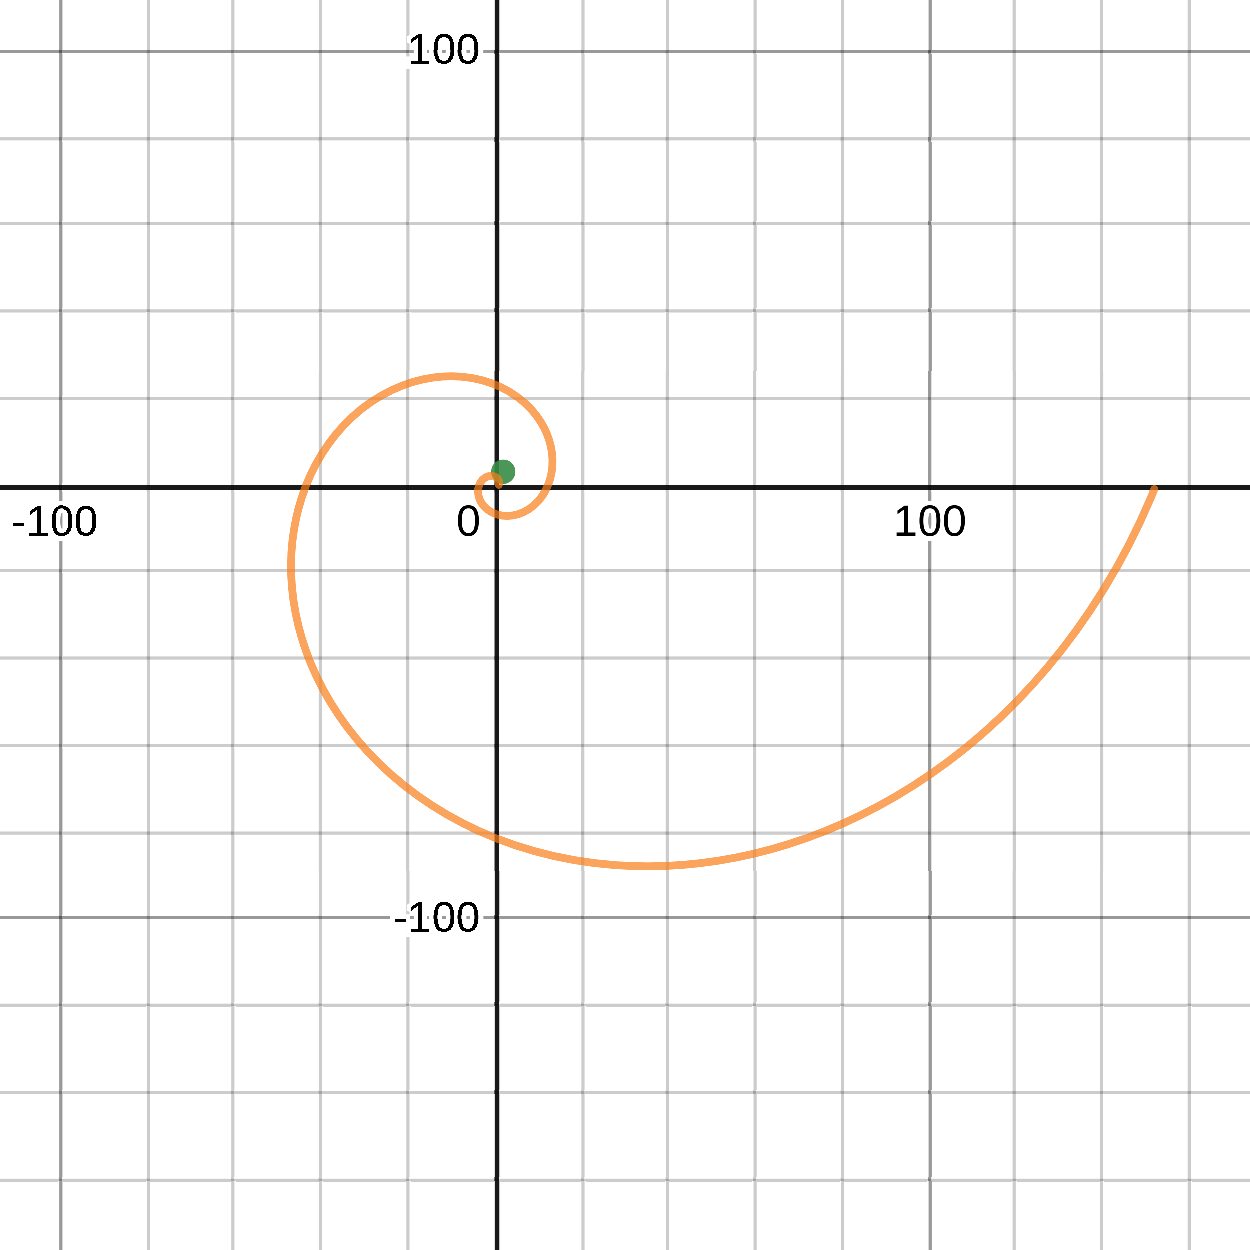
\includegraphics[scale=0.5]{desmos-graph}
\par\end{center}

\begin{flushleft}
Vamos, primero, a calcular la longitud de la curva entre $t_{0}$
y $t_{1}$. O sea
\[
L_{t_{0}}^{t_{1}}\left(\alpha\right)=\int_{t_{0}}^{t_{1}}\left|\alpha'\left(s\right)\right|ds
\]
\par\end{flushleft}

\begin{flushleft}
Ahora bien
\[
\alpha'\left(t\right)=a\cdot e^{bt}\left(bcos\left(t\right)-sen(t),bsen\left(t\right)+cos\left(t\right)\right)
\]
 por lo que
\[
\left|\alpha'\left(t\right)\right|=\sqrt{a^{2}\cdot e^{2bt}\left(b^{2}cos^{2}t+sen^{2}t-2b\cdot cost\cdot sent+b^{2}sen^{2}t+cos^{2}t+2b\cdot cost\cdot sent\right)}=
\]
\[
=a\cdot e^{bt}\sqrt{b^{2}+1}
\]
 es decir
\[
L_{t_{0}}^{t_{1}}\left(\alpha\right)=\int_{t_{0}}^{t_{1}}a\cdot e^{bt}\sqrt{b^{2}+1}dt=\left[\frac{a}{b}\cdot\sqrt{b^{2}+1}e^{bt}\right]_{t_{0}}^{t_{1}}=\frac{a}{b}\sqrt{b^{2}+1}\left(e^{bt_{1}}-e^{bt_{0}}\right)
\]
\par\end{flushleft}

\begin{flushleft}
Por el teorema 1.1.7, sabemos que existe una reparametrizaci�n por
la longitud de arco, y que viene dado por la inversa de 
\[
s=g\left(t\right)=\int_{0}^{t}\left|\alpha'\left(u\right)\right|du=\frac{a}{b}\sqrt{b^{2}+1}\left(e^{bt}-1\right)
\]
\par\end{flushleft}

\begin{flushleft}
As�, despejamos $t$:
\[
\frac{s\cdot b}{a\sqrt{b^{2}+1}}=e^{bt}-1\implies\frac{s\cdot b}{a\sqrt{b^{2}+1}}+1=e^{bt}\implies log\left(\frac{s\cdot b}{a\sqrt{b^{2}+1}}+1\right)=bt\implies
\]
\[
\implies t=h\left(s\right)=\frac{1}{b}log\left(\frac{s\cdot b}{a\sqrt{b^{2}+1}}+1\right)
\]
\par\end{flushleft}

\begin{flushleft}
De esta manera, la reparametrizaci�n buscada es:
\[
\beta\left(s\right)=\alpha\left(h\left(s\right)\right)=ae^{log\left(\frac{s}{a\sqrt{b^{2}+1}}+1\right)}\left(cos\left(\frac{1}{b}log\left(\frac{sb}{a\sqrt{b^{2}+1}}+1\right)\right),sen\left(\frac{1}{b}log\left(\frac{sb}{a\sqrt{b^{2}+1}}+1\right)\right)\right)=
\]
\[
=a\left(\frac{sb}{a\sqrt{b^{2}+1}}+1\right)\left(cos\left(\frac{1}{b}log\left(\frac{sb}{a\sqrt{b^{2}+1}}+1\right)\right),sen\left(\frac{1}{b}log\left(\frac{sb}{a\sqrt{b^{2}+1}}+1\right)\right)\right)
\]
\par\end{flushleft}

\begin{flushleft}
Para ver que, efectivamente, esto es la reparametrizaci�n correcta,
debemos comprobar que $\left|\beta'\left(s\right)\right|=1,\ \forall s$.
\par\end{flushleft}

\begin{flushleft}
Siendo
\[
\beta'\left(s\right)=\frac{1}{\sqrt{b^{2}+1}}\left(\beta'_{x},\beta'_{y}\right)
\]
\[
\beta'_{x}=b\cdot cos\left(\frac{log\left(\frac{bs}{a\sqrt{b^{2}+1}}+1\right)}{b}\right)-sen\left(\frac{log\left(\frac{bs}{a\sqrt{b^{2}+1}}+1\right)}{b}\right)
\]
\par\end{flushleft}

\[
\beta'_{y}=b\cdot sen\left(\frac{log\left(\frac{bs}{a\sqrt{b^{2}+1}}+1\right)}{b}\right)+cos\left(\frac{log\left(\frac{bs}{a\sqrt{b^{2}+1}}+1\right)}{b}\right)
\]

\begin{flushleft}
Y su norma, llamando $z:=\frac{log\left(\frac{bs}{a\sqrt{b^{2}+1}}+1\right)}{b}$
\[
\left|\beta'\left(s\right)\right|=\frac{1}{\sqrt{b^{2}+1}}\sqrt{b^{2}cos^{2}z+sen^{2}z-2b\cdot cosz\cdot senz+b^{2}sen^{2}z+cos^{2}z+2b\cdot senz\cdot cosz}=\frac{\sqrt{b^{2}+1}}{\sqrt{b^{2}+1}}=1
\]
\par\end{flushleft}
\end{document}
